%  A simple AAU report template.
%  2013-03-06 v. 1.0.0
%  Copyright 2010-2013 by Jesper Kjær Nielsen <jkn@es.aau.dk>
%
%  This is free software: you can redistribute it and/or modify
%  it under the terms of the GNU General Public License as published by
%  the Free Software Foundation, either version 3 of the License, or
%  (at your option) any later version.
%
%  This is distributed in the hope that it will be useful,
%  but WITHOUT ANY WARRANTY; without even the implied warranty of
%  MERCHANTABILITY or FITNESS FOR A PARTICULAR PURPOSE.  See the
%  GNU General Public License for more details.
%
%  You can find the GNU General Public License at <http://www.gnu.org/licenses/>.
%
\pdfbookmark[0]{Front page}{label:frontpage}%
\begin{titlepage}
  \addtolength{\hoffset}{0.5\evensidemargin-0.5\oddsidemargin} %set equal margins on the frontpage - remove this line if you want default margins
  \noindent%
  %\vspace{4cm}
  \begin{tabular}{@{}p{\textwidth}@{}}
    %\vspace{5cm}
    \toprule[2pt]
    \midrule
    \vspace{0.4cm}
    \begin{center}
    \Huge{\textsc{An introductory examiniation of the Finite Element Method}}
    \end{center}
  %  \\
    \vspace{0.4cm}\\
    \midrule
    \toprule[2pt]
  \end{tabular}
  \vspace{0.8cm}
  \setlength\fboxsep{0pt}
    \begin{figure}[ht]
        \centering
      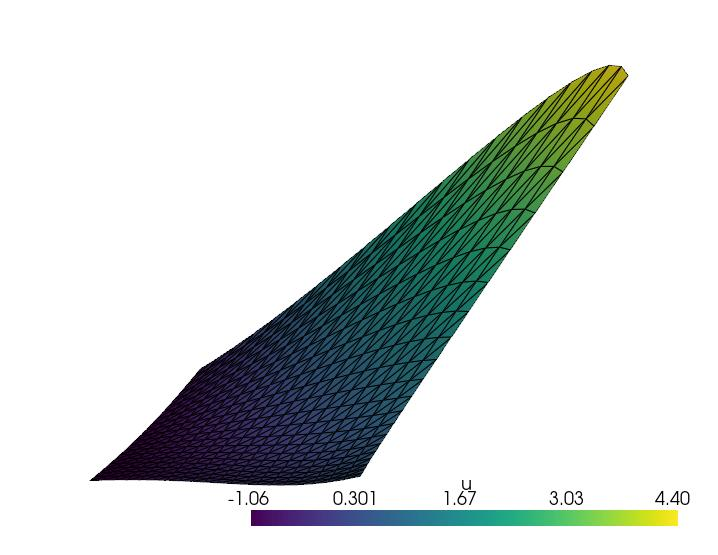
\includegraphics[width=\textwidth]{Afsnit/Application/figurer/screenshot_3.jpeg}
    \end{figure}
    \setlength\fboxsep{5pt}
  %\begin{center}
    % {Projektrapport 3. semester%Insert document type (e.g., Project Report)
    % }\\
    % \vspace{0.2cm}
    % {Gruppe 4.211%Insert your group name or real names here
    % }
  %\end{center}
  \vfill
\begin{center}
  {\large{Group 5.216c} \\
    {Aalborg University} \\
    {Mathematics} \\}
\end{center}
  
%   \begin{center}
%   Aalborg Universitet\\
%   Institut for Matematiske Fag\\
%   Skjernvej 4A\\
%   DK-9220 Aalborg Øst
%   \end{center}
\end{titlepage}
\clearpage

\thispagestyle{empty}
{\small
\strut\vfill % push the content to the bottom of the page
\noindent Copyright \copyright{} Aalborg University 2024\par
\vspace{0.2cm}
%\noindent Here you can write something about which tools and software you have used for typesetting the document, running simulations and creating figures. If you do not know what to write, either leave this page blank or have a look at the colophon in some of your books.
}
\clearpage
